% Created 2020-11-17 二 20:49
% Intended LaTeX compiler: xelatex
\documentclass[11pt]{article}
\usepackage{graphicx}
\usepackage{grffile}
\usepackage{longtable}
\usepackage{wrapfig}
\usepackage{rotating}
\usepackage[normalem]{ulem}
\usepackage{amsmath}
\usepackage{textcomp}
\usepackage{amssymb}
\usepackage{capt-of}
\usepackage{hyperref}
\usepackage{ctex}
\author{Wang Jian}
\date{\today}
\title{Gee PS: Scalable deep learning on distributed GPUs with a GPU-specialized parameter server}
\hypersetup{
 pdfauthor={Wang Jian},
 pdftitle={Gee PS: Scalable deep learning on distributed GPUs with a GPU-specialized parameter server},
 pdfkeywords={},
 pdfsubject={},
 pdfcreator={Emacs 27.1 (Org mode 9.4)}, 
 pdflang={English}}
\begin{document}

\maketitle
\tableofcontents

\section{Author}
\label{sec:org4817a46}
\url{https://cuihenggang.github.io/}

\section{Notes on a paper:}
\label{sec:orga8658d2}
GeePS is a smart data manager (data migration/movement coordinator) for a very large distributed deep learning training on GPUs. The paper addressed a real need and showed how a problem of distributed learning with GPUs can be solved.

\subsection{Tree primary contributions:}
\label{sec:org341cfb5}
\begin{enumerate}
\item it describes the first GPU-specialized parameter server design and the changes needed to achieve efficient data-parallel multimachine deep learning with GPUs.
\item it reports on large-scale experiments showing that GeePS indeed supports scalable data parallel execution via a parameter server, in contrast to previous expectations [7].
\item it introduces new parameter server support for enabling such data-parallel deep learning on GPUs even when models are too big to fit in GPU memory, by explicitly managing GPU memory as a cache for parameters and intermediate layer state
\end{enumerate}
\subsection{Background}
\label{sec:orgbae0c45}
\begin{enumerate}
\item Deep learning with GPUs
\item Parallel ML using PS
\item \textbf{MXNet uses ParameterServer which is CPU-based parameter server}
\end{enumerate}
\subsection{Design}
\label{sec:orgd3abe9f}
As mentioned earlier, GeePS shards the parameters across the machines. The parameters are stored as an array of fixed size called rows and each row is associated with a key. Rows are bundled together into tables and each table stores information like data age, which denotes how many times the values in the table has updated and requires a refresh.

In addition to this each instance has a parameter cache, local data and access buffer pool. Parameter cache(write back) caches all parameters of the NN in GPU( can be overflowed to CPU memory). This reduces the communication overhead during an iteration. Local data (also stored in GPU \& CPU) are the additional memory needed for intermediate states. This is local to the machine and not shared across the cluster. Access buffer pool is used when application makes read and update calls. GeePS first allocates a buffer in GPU memory and copies the data to it before letting application to read or write to that buffer. This ensures data consistency.

\begin{center}
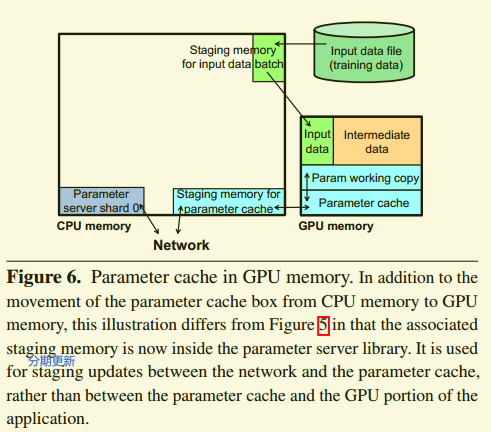
\includegraphics[width=.9\linewidth]{GeePS.org_imgs/20201117_203549_laJAue.png}
\end{center}
\subsection{Implementation}
\label{sec:org17bc915}
GeePS prebuilts the indexes based on the details collected during a dry run before the actual training starts. Since NNs computations are repetitive this information is not going to change. During the training iteration, the application reads and updates the parameters on individual machines and at the end GeePS triggers a TableClock. This signals all machines to synchronize the data based on the BSP or SSP policies. The data transfer between machines is done using 3 threads, keeper, pusher and puller. Pusher pushes updates from the master machines(of a set of parameters) to other machines to cache. Keeper receives this updates and forward it to Puller for updated GPU cache.

The data allocation and reclamation is also done using 2 threads called allocator and reclaimer. These threads synchronize each other with mutex locks on parameter partitions. GeePS avoid using row level fine grained locking. Usually there is only one CPU thread interacting with GeePS and the lock contention is not a big deal.
\subsection{Evaluation results}
\label{sec:orgdf9e3fa}
GeePS is evaluated against image classification workloads. It provides 13x improvement in throughput using 16 GPUs. Less than 8\% of the time is lost to GPU stalls as compared to CPU based parameter server. GeePS gets same throughput as ProjectAdam, a state of the art CPU based distributed deep learning solution using 108 machines, with only 4 GPUs.
\end{document}
